\chapterimage{anhang.png}
\chapter{Anhang}
\label{chap:appendix}

\section{Anhang 1: Fragebogen}
\label{anhang:fragebogen}
\\\\---->TODO: Formular\\\\

\section{Anhang 2: Personas}
\label{anhang:personas}
\\\\---->TODO: Welche Personae kommt hier?\\\\

\section{Anhang 3: Prototypen}
\label{anhang:protos}
Dieses Anhang enthält alle prototypen im größere Forme, damit der Leser detailierte blick auf alle Features haben kann.

\begin{figure}[ht]
    \centering
      \makebox[\textwidth]{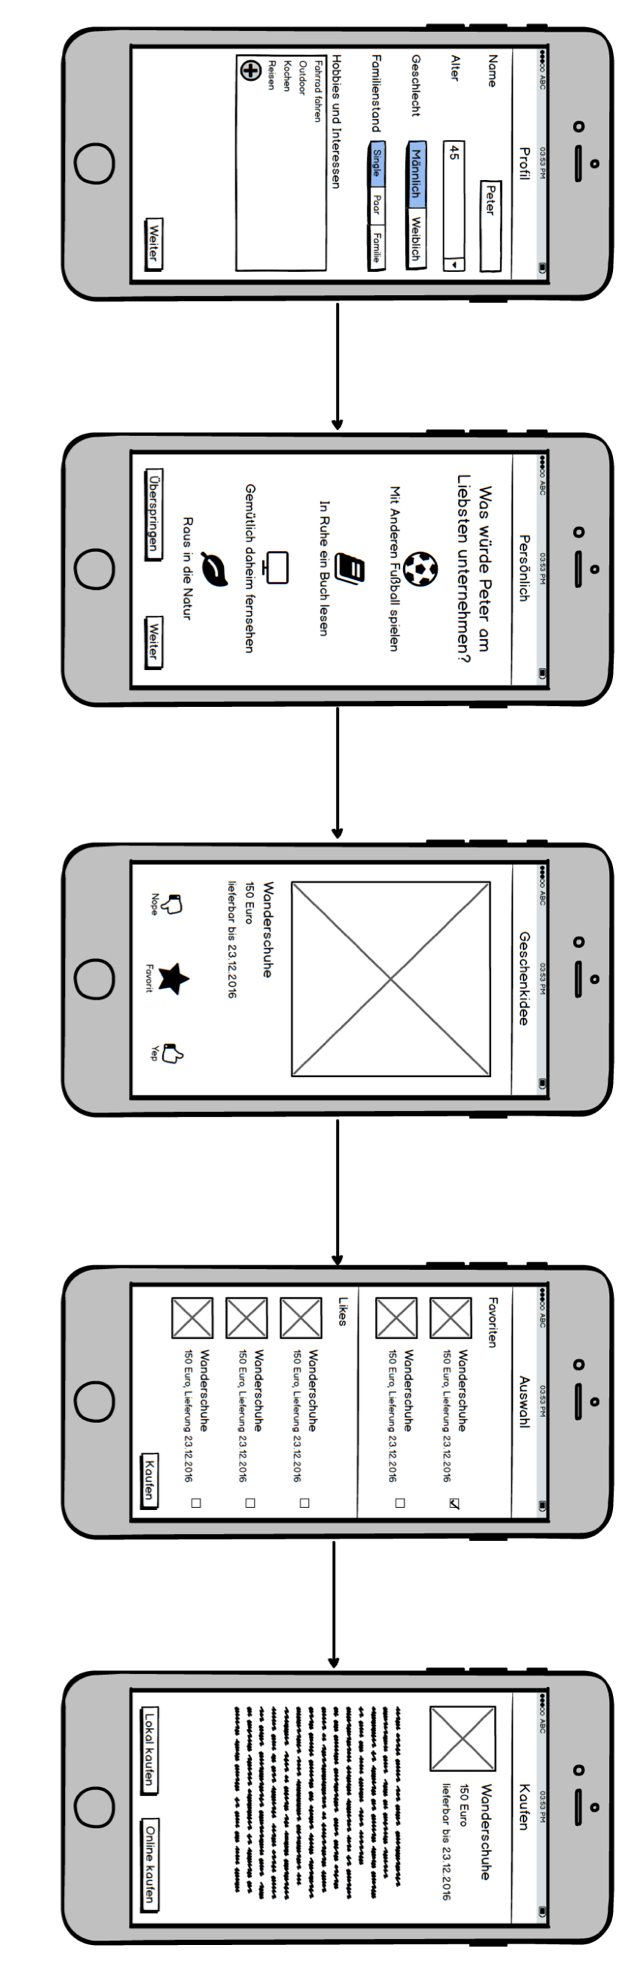
\includegraphics[height=0.83\paperheight]{prt1}}
    \caption{Swipe-App (Prototyp 1)}
    \label{fig:prt1}
\end{figure}

\begin{figure}[ht]
    \centering
      \makebox[\textwidth]{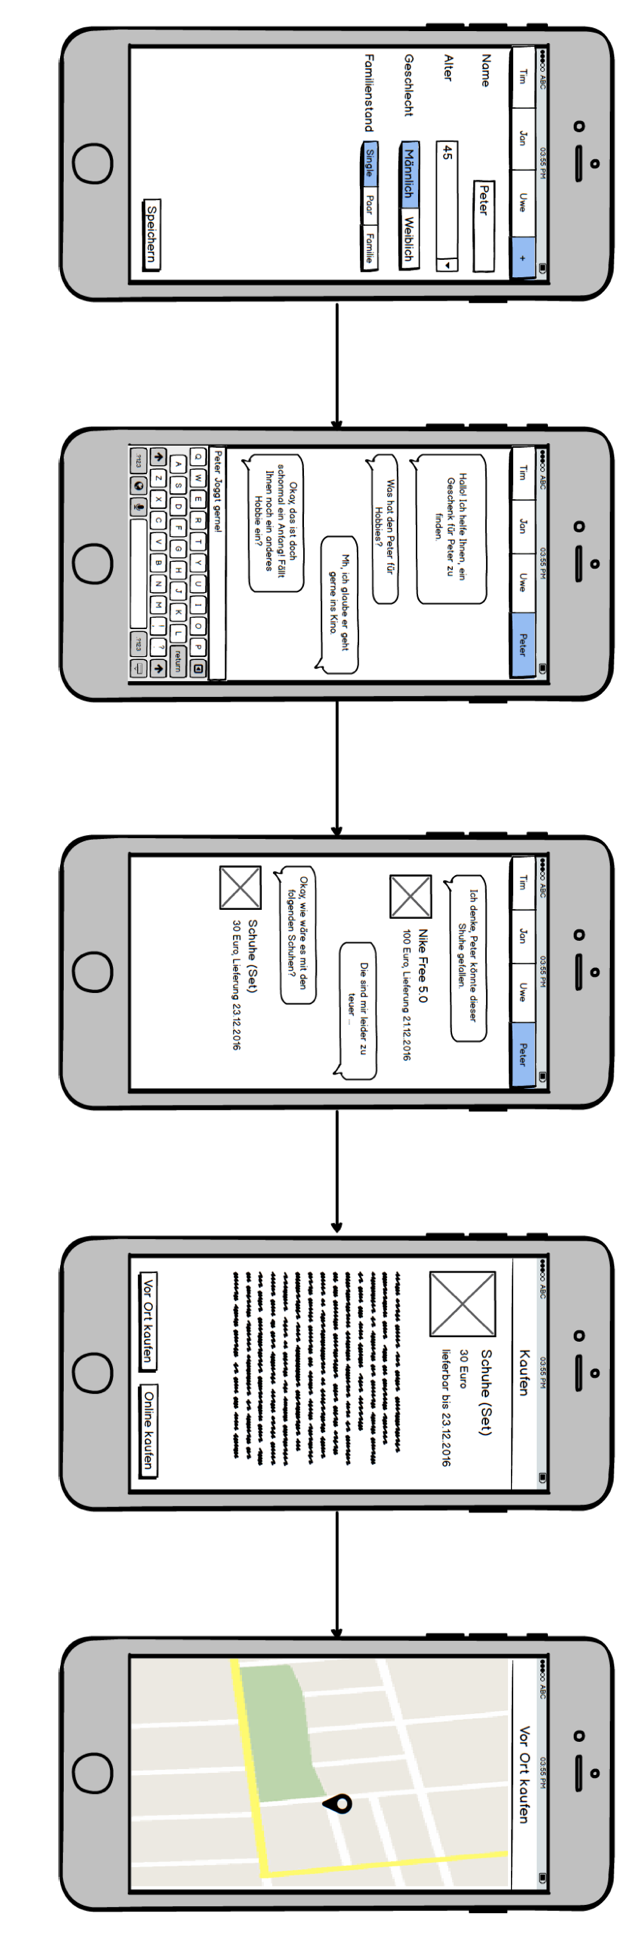
\includegraphics[height=0.83\paperheight]{prt2}}
    \caption{Chat-Bot (Prototyp 2)}
    \label{fig:prt2}
\end{figure}

\begin{figure}[ht]
    \centering
      \makebox[\textwidth]{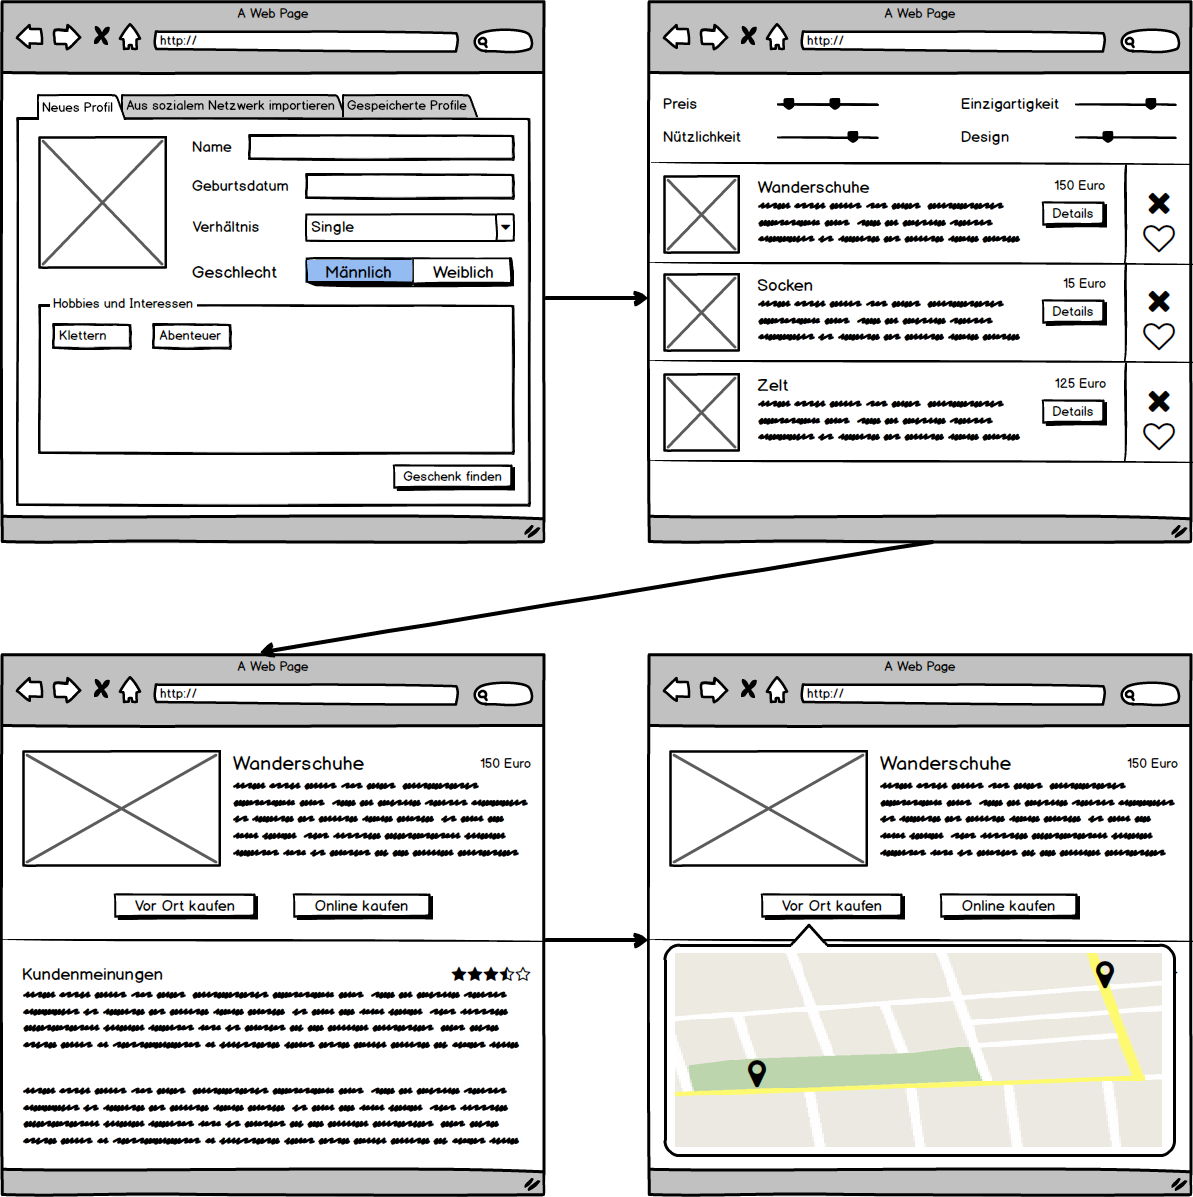
\includegraphics[width=0.83\paperwidth,height=0.65\paperheight]{prt3}}
    \caption{Webseite (Prototyp 3)}
    \label{fig:prt3}
\end{figure}

\begin{figure}[ht]
    \centering
      \makebox[\textwidth]{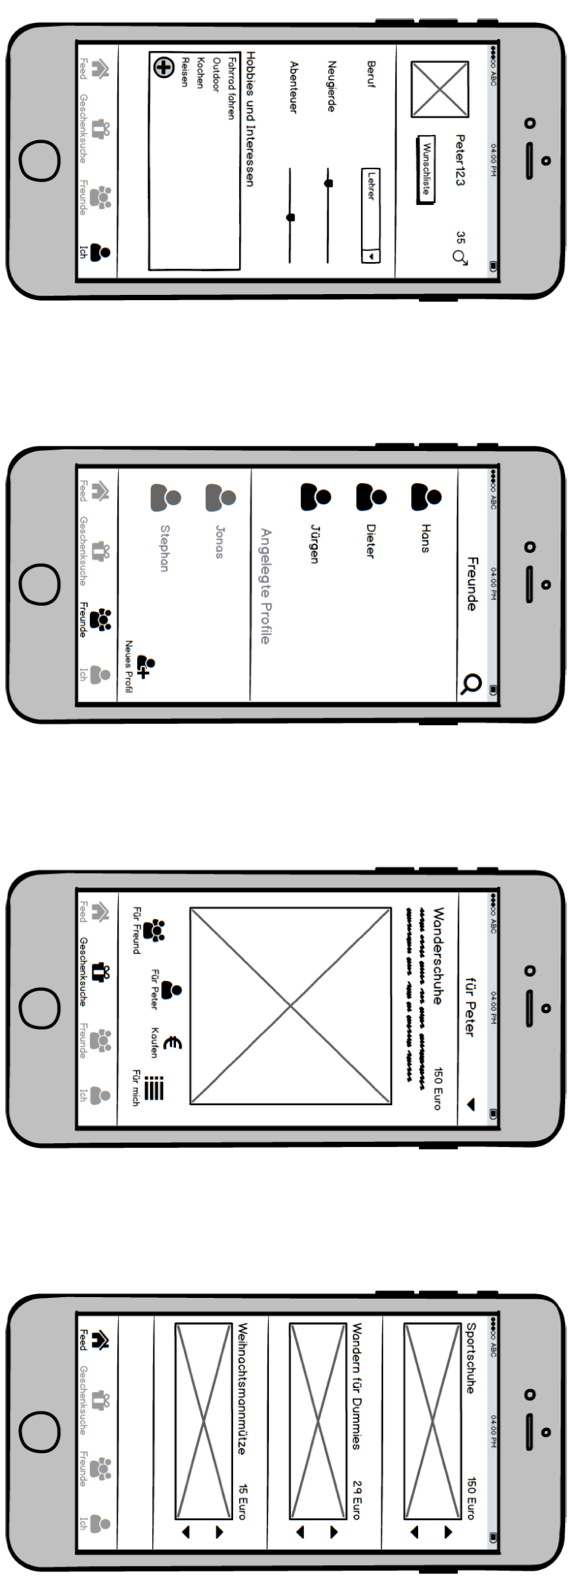
\includegraphics[height=0.8\paperheight]{prt4}}
    \caption{Soziales Netz (Prototyp 4)}
    \label{fig:prt4}
\end{figure}
